\documentclass{siproblemset}

% SI Session Information
\course{MTH 1321}       % the course of your SI
\sessionnum{15}         % (optional) specify the session number
\sessiondate{3/30/21}   % the date of the session

\warmup{Concept Review}
\topic{Concavity}
\topic{Points of Inflection}
\topic{Second Derivative Test}
\cooldown{Extrema from Graphs}

% Worksheet Information
\title{The Second Derivative\linebreak Test and Concavity}
\sections{Section 4.4}
\withnamespace

\begin{document}
    \maketitle
    
    \activity{Activity 1}{Second Derivative Test}{Work together in your \textbf{breakout rooms} to answer these questions. Do your best to not refer to your notes while working on these problems.}{30 minutes}
    
    \mcq{For the following functions, (a) find the critical points and, (b) if possible, use the Second Derivative Test to classify them as local minimums, local maximums, or neither. If the Second Derivative Test is inconclusive, state so explicitly and use another method.}{
        \task $f(x)=2x^4-3x^2+2$
        \largesp
        \task $g(x)=(x^2-2)e^{-x}\hspace{0.5cm}$
    }
    \newpage

    \activity{Activity 2}{Concavity and Points of Inflection}{Work together in your \textbf{breakout rooms} to answer these questions. Do your best to not refer to your notes while working on these problems.}{30 minutes}
    
    \mcq{For the following functions, (a) find the inflection points and, (b) determine the intervals of concavity.}{
        \task $f(t)=t^3-6t^2+4$
        \Largesp
        \task $y=\theta-2\sin\theta\hspace{0.5cm}[0, 2\pi]$

    }
\newpage
    
    
    \mcq[2]{The following graph is the graph of $f'$, the derivative of the twice-differentiable function $f$. Determine the following:}{
        \task The $x$-values of local extrema
        \task The $x$-values of inflection points
        \task Intervals of increase and decrease of $f$
        \task Intervals where $f$ is concave up and down
    }
    
    \begin{center}
        \mbox{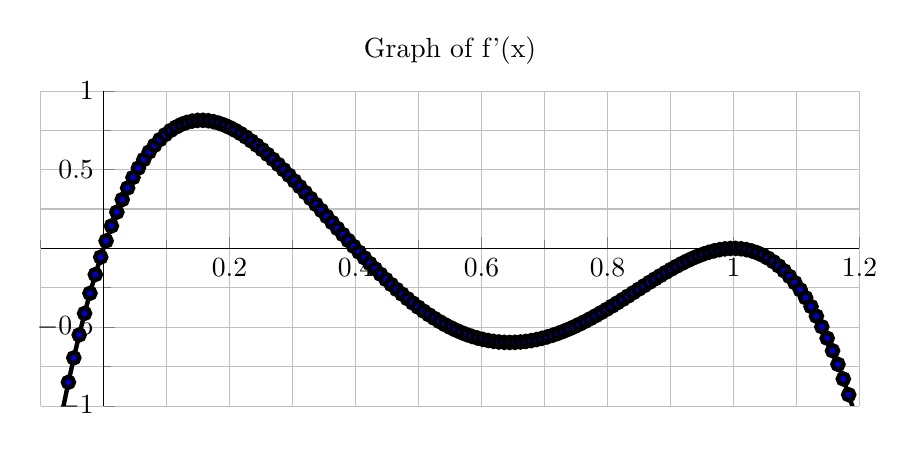
\begin{tikzpicture}[baseline=(current bounding box.north)]
            \begin{axis}[
            title={Graph of f'(x)},
            x=8cm,
            y=2cm,
            xmin=-0.1,
            xmax=1.2,
            ymin=-1,
            ymax=1,
            grid=both,
            major grid style={line width=.2pt,draw=gray!50},
            minor tick num=1,
            axis x line*=middle,
            axis y line*=middle,
            every axis plot/.append style={ultra thick},
            samples=200
            ]
            \addplot+[black, domain=-0.5:1.2] {-30*x*(x-0.4)*(x-1)^2};
            \end{axis}
            \end{tikzpicture}}
    \end{center}

\newpage
    
    \activity{Cooldown}{Determining the Behavior of a Function from a Table}{Do this problem \textbf{alone}.}{15 minutes}
    
    \begin{multipartquestion}
        Use the table below to answer parts (a)–(e). Assume that $f$ is a well-behaved twice-differentiable function.
        \begin{center}
            \begin{tabular}{|c|c|c|c|c|c|c|c|}
                \hline
                $x$ & 1 & 2 & 3 & 4 & 5 & 6 & 7 \\
                \hline
                $f(x)$ & -3 & 0 & 4 & -2 & 9 & 2 & -4 \\
                \hline
                $f'(x)$ & -3 & 1 & 0 & DNE & 2 & 0 & -1 \\
                \hline
                $f''(x)$ & 3 & 0 & 2 & 1 & 0 & -1.5 & -3\\
                \hline
            \end{tabular}
        \end{center}
        
        \frq{What are the critical points of $f$?}
        \tinysp
        \frq{At what $x$-values is $f$ increasing and decreasing?}
        \tinysp
        \frq{At what $x$-values is $f$ concave up and down?}
        \tinysp
        \frq{Estimate which $x$-values correspond to local extrema.}
        \tinysp
        \frq{Estimate which $x$-values correspond to points of inflection.}
        \tinysp
        
    \end{multipartquestion}
    
\end{document}